\section{Background}

A species phylogeny is a graphical model of the common evolutionary history of a group of species, and is most often represented as a phylogenetic tree  or phylogenetic network 
\cite{MorrisonNetworks}.
A species phylogeny 
gives valuable information about protein functions
\cite{Sjolander-function,Eisen-phylogenomics,ProteinFunctions},   host-parasite relationships \cite{CoEvolution}, etc.

However, species tree estimation is difficult, 
due to multiple biological processes, including
recombination \cite{TheCell}, duplication 
and loss \cite{GeneticsInMedicine}, hybridization \cite{NaturalHybridization}, 
incomplete lineage sorting (ILS) \cite{Maddison}, 
and horizontal gene transfer (HGT) \cite{Woese2002},
that can cause
a given genomic locus  to have
a tree that is different from the species
tree.
As a result, multiple loci are needed to estimate
a species
phylogeny with high accuracy. 



Of the many sources of gene tree discord, the one
that has received the greatest attention is ILS,
which is
modeled by the multi-species coalescent (MSC) model \cite{Kingman82}.
An MSC model tree has a rooted tree $T$, leaf-labelled
by  a set of species,  and is given with branch lengths in
coalescent units. Gene trees evolve
within the species tree, in a backwards 
process described by the MSC; thus, lineages ``coalesce" on the branches of the tree,
as they move from the leaves of the species tree towards the root.
When two lineages fail to coalesce on the earliest branch in which they
can coalesce, this can result in a gene tree having a different
topology than the species tree.

Under the MSC model, each species tree defines a probability distribution on
gene trees, and the species tree can be identified uniquely from
this distribution. Hence, one type of technique (called
a ``summary method") for estimating
species trees under the MSC operates by first estimating gene trees
for a set of different loci, and then uses this estimated distribution on
gene trees to
estimate the species tree. 
A summary method is said to be statistically consistent
under the MSC model if, 
as the number of loci and sites per locus go to infinity, 
the estimated species tree returned by the method will converge 
in probability to the true species tree \cite{WarnowCurrents2015}.
Many statistically 
consistent summary methods have been developed for estimating species trees 
when gene discordance is due to ILS 
\cite{mpest,Mossel2010,stem,star,njst,Astral,Astral2}. 

Despite advances in
developing statistically
consistent methods for species tree
estimation that are robust to ILS,
by far the  most common technique for estimating a species tree
is 
concatenation analysis,
in which the sequence alignments for the
different loci are combined into one
large supermatrix, and then a phylogeny is
estimated on the alignment using maximum likelihood \cite{JarvisScience2014,1kp}.
This type of approach, however, 
 is sometimes  not statistically consistent under the multi-species coalescent
model \cite{RochSteel,WarnowCurrents2015}
in the presence of ILS. 
Hence, even though concatenation
often has good accuracy (even under conditions with moderately 
high ILS levels) \cite{GatesySpringer,patel2013error,naive-binning},
a large effort has been made to develop 
alternative methods that are provably robust to ILS and
have good accuracy on realistic conditions.

For very small datasets, 
Bayesian
methods such as 
BEST \cite{best}, 
*BEAST \cite{Heled2010} or BUCKy-pop \cite{Larget2010} 
(the population tree from BUCKy)  can provide
excellent accuracy; however, these methods are too
computationally intensive to use on even moderate sized datasets
with hundreds to thousands of loci and 30 or more species \cite{Zimmermann2014,YangWarnow}. 




Of the currently available coalescent-based methods, 
ASTRAL-2 \cite{Astral2}, MP-EST \cite{Liu2010a},
and NJst \cite{liu2011estimating} have emerged as the most
accurate of the methods that
can run 
on datasets with 50 or more species and hundreds to thousands
of loci. 
However, the comparison among these methods shows that MP-EST is
typically not as accurate as NJst and ASTRAL-2
and is also much slower than both   \cite{Astral2}.
Some newer statistically consistent
methods
have also been developed
(e.g., SVDquartets \cite{chifman2014quartet}), but have not 
%Jun17 - small addition below
yet been sufficiently evaluated in terms of their accuracy and
scalability in comparison to
other coalescent-based methods.

Some of the most commonly used coalescent-based
methods estimate
species trees by encoding each gene tree as a set of quartet
trees (i.e., 
unrooted 4-leaf trees), and then estimate the species tree from
the quartet tree frequencies.
The mathematical  basis of this approach
is the following theorem, originally proved in \cite{AllmanDegnanRhodes2011a}:
\begin{theorem}
Under the multi-species coalescent model, 
for every
model 
species tree $T,\theta)$
(where $\theta$ denotes the branch lengths of $T$ in
coalescent units) and for every
set $X$ of
four leaves from $T$,  the most probable
unrooted
gene tree topology on $X$ is identical to the
species tree $T$ restricted to leafset $X$.
\label{hgt::theorem1}
\end{theorem}

Interestingly, nearly the same theorem was proven
under two phylogenomic models that addressed
horizontal gene transfer (HGT)!
When HGT is
present,  the evolutionary history of the species is 
not really treelike, but rather requires a 
phylogenetic network  \cite{MorrisonNetworks}. 
Under HGT models, 
a phylogenetic network  consists of
an underlying species tree $T$ with 
horizontal gene transfer
edges (represented by directed edges)  between 
branches in the tree, and
each locus evolves down a tree (though not
necessarily the species tree) within this network.
Hence, while the species evolution is not purely treelike, 
the gene tree evolution {\em is} treelike. 
Furthermore, for this type of reticulate phylogeny,
it is reasonable to ask whether the underlying species tree 
$T$
can be
reconstructed from gene trees estimated on the different
loci. 
 
This question has been partially answered for
two models of HGT.
The first models  HGT events between lineages 
using a continuous-time Poisson process \cite{Galtier07}, and
is called the
\emph{stochastic HGT model}. 
In a stochastic HGT model, the 
HGT events happen between contemporaneous lineages,
either uniformly at randomly or with probability that depends on the distance between the lineages
(so that events are less likely if the lineages are more distantly related).
The second type of model assumes that there are HGT edges 
between specific pairs of branches in a species tree, 
commonly referred to as \emph{highways}, 
along which HGT events are far more likely to occur than elsewhere in 
the tree;
this is called the
  \emph{highways HGT model} \cite{BeikoHighways}. 

The theoretical framework for estimating the underlying
species tree under these two HGT models was established in
\cite{SteelLGT1} (for estimating rooted species trees from
rooted gene trees) and in \cite{RochSnir} (for
estimating unrooted species trees from unrooted gene trees).
Specifically,
 \cite{RochSnir} proved theorems that
under both the stochastic HGT model and highways
model, but with
bounded amounts of HGT per gene,
the most probable quartet
tree would be topologically identical to the species tree.
Note that these
theorems are  the equivalents of Theorem \ref{hgt::theorem1}
under the two bounded HGT models. 

Some  species tree estimation methods 
operate by computing gene trees, encoding each computed
gene tree as a set of quartet trees, and determine the
dominant quartet tree for every four species (i.e., the
quartet tree that appears the most frequently of the 
three possible unrooted quartet trees).
Then, these 
dominant quartet trees are combined using
a quartet amalgamation method
(e.g., Quartets Max Cut \cite{qmc} or QFM \cite{reaz2014accurate}).
This type of species tree estimation method 
can be statistically consistent under
the MSC model, and also under these bounded HGT models --
depending on the quartet amalgamation method, as we now show.
\begin{theorem}
\label{hgt::thm:astral-stat-hgt}
Let $M$ be a summary method  (i.e., a method that
constructs a species tree from an input set of gene trees).
Suppose that $M$ has the property that
it is guaranteed to return the unique tree
compatible with the dominant quartet trees defined
by its input set of gene trees, whenever
the dominant quartet trees are compatible.
Then $M$ is
statistically consistent under the 
MSC model, and also 
under the bounded HGT models 
given in \cite{RochSnir}.
\end{theorem}
\begin{proof}
To establish statistical consistency, we only need to
prove that as the number of sites per locus and the number of loci
both increase, the tree returned by the method converges
in probability
to the species tree. 
As the number of sites per locus and the number of
loci both increase, the dominant quartet tree converges to the
most probable quartet tree on every set $X$ of four species. 
Under the MSC model and also
under the bounded HGT models in \cite{RochSnir},
the most probable quartet tree on any set $X$ is
topologically identical to the species tree.
Hence, for a large enough number of loci and large enough
number of sites per locus, with probability converging to $1$, the
input to the quartet-based methods 
will be a set of gene trees such that the dominant
quartet trees are all compatible with the species tree.
Furthermore, the species tree will be the
unique such compatibility tree, and so
the method will return the true species tree.
\end{proof}


%Ruth: removed word "sketch"
Similarly, we can prove the following:
\begin{theorem}
ASTRAL and ASTRAL-2  are statistically consistent under the bounded
HGT models of \cite{RochSnir}. 
\label{hgt::theorem-corollary}
\end{theorem}
This proof uses Theorem \ref{hgt::theorem1}, 
but is essentially identical to the proofs of
statistical consistency for ASTRAL and ASTRAL-2 under
the MSC model \cite{Astral2}; see Methods for
the proof of this theorem.


%In this paper we investigate the evaluation of species tree estimation methods in the presence of HGT and ILS.  This is an important problem to investigate because if a species tree estimation method is designed to return accurate trees in the presence of ILS, examining its performance in the presence of both ILS and HGT amounts to examining its tolerance to a specific type of model misspecification. 

Very little is known about the
theoretical guarantees of any
species tree estimation methods under
models in which both HGT and ILS can occur.
In fact, to the best of our knowledge,
no methods have yet been proven statistically
consistent under these conditions.
We also do not know much about the empirical performance of
any species tree estimation methods under
these conditions.
As far as we know, the only simulation study to 
date of the impact of both ILS and HGT on 
the performance of species tree estimation methods is \cite{ChungAne},
which   explored  the performance of two coalescent-based methods, 
BUCKy  and BEST, on data that evolved 
under both processes. 
However, both
of these methods are computationally 
intensive, and cannot run on even moderately
large datasets
%Jun17: I removed the following phrase because BUCKy *can* 
%           run on datasets of 20 species and 100 genes. Either don?t give 
%          exact numbers, or give them based on a prior study. The numbers 
%          are too low for BUCKy. Note in our ASTRAL paper, we ran BUCKy 
%         on 37 taxa and 400 genes.  
% containing 20 or more species and hundreds or thousands of loci
(e.g., BEST is slower than *BEAST, and *BEAST is
too computationally intensive to use on datasets with
more than about 100 loci)
\cite{YangWarnow,Zimmermann2014}.








We report
on a study evaluating
the accuracy  of 
ASTRAL-2, NJst, and 
weighted Quartets Max Cut (wQMC) \cite{wQMC}, as
well as  unpartitioned maximum likelihood concatenation analysis (CA-ML), 
on simulated datasets in which
gene tree discord is due to both HGT and ILS.
The simulation protocol evolved
gene trees down 50-taxon species trees under the MSC model with a moderately
high level of ILS, and allowed gene trees to then evolve with 
six different HGT rates (see Fig.~\ref{hgt::sim}). 
HGT rate (1) has no  HGT  events,
and 
HGT rates (2)-(6) have 0.08, 0.2, 0.8, 8.0, and
20.0  expected HGT events per gene, respectively.
Finally, sequences evolved down each gene tree under the GTR+Gamma model.

  \begin{figure}
\centering
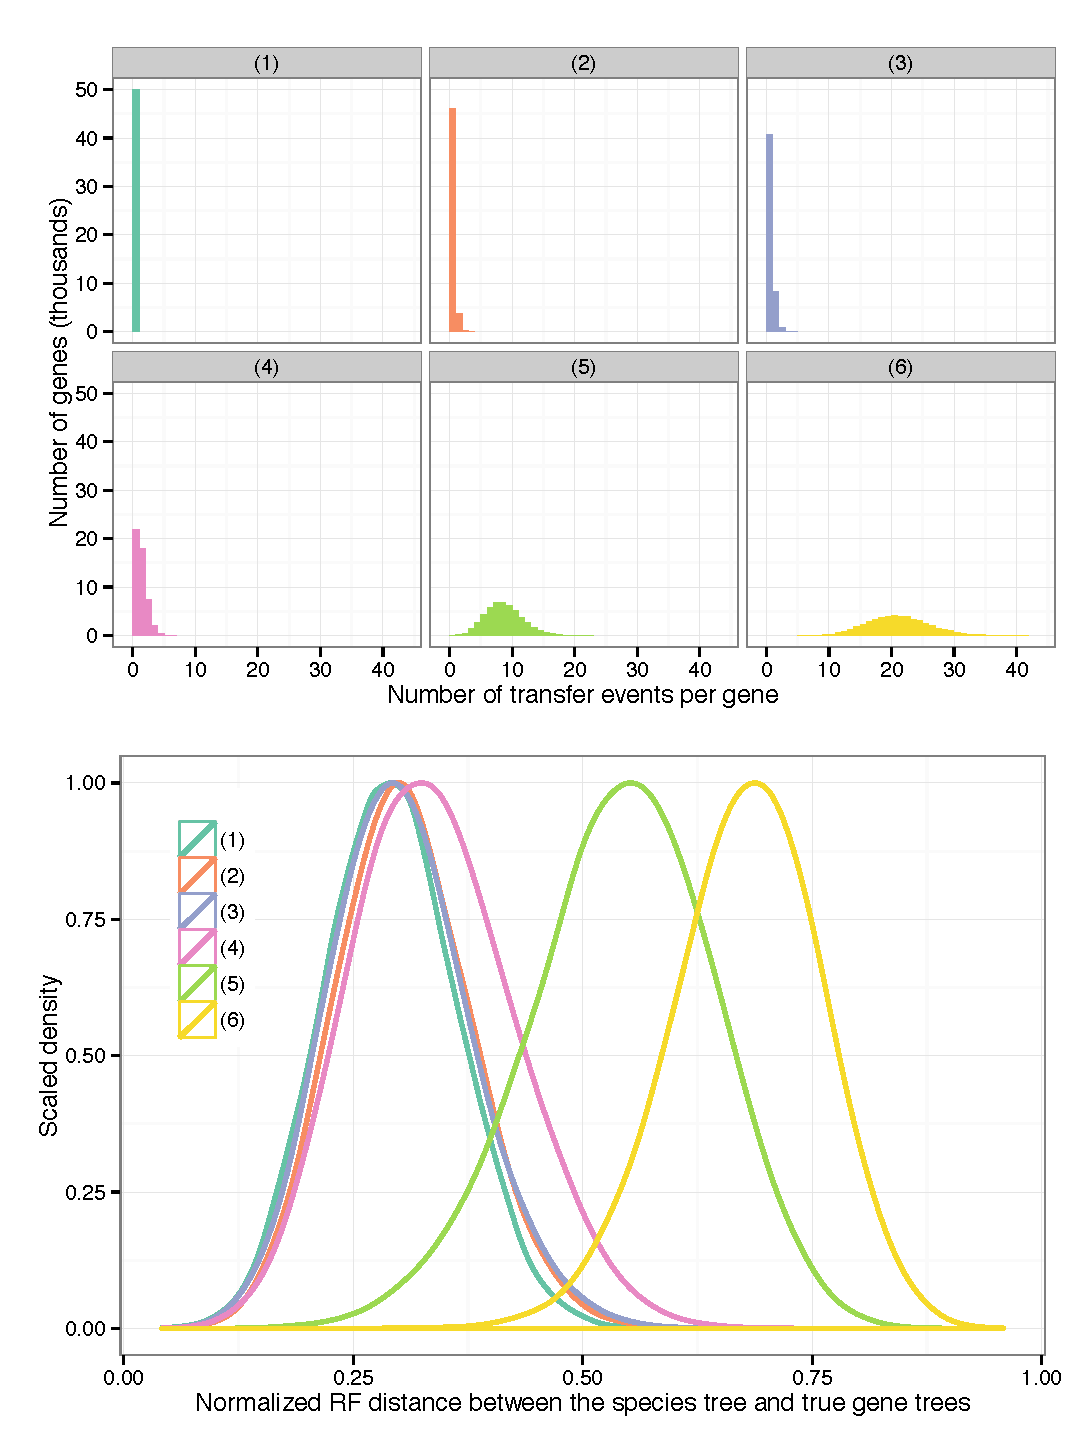
\includegraphics[width=12cm]{hgt-figs/both.eps}
 \caption[Properties of simulated datasets for HGT+ILS study]{{\bf Properties of the simulated datasets.  } 
(Top) The histogram of the number of transfer events per gene across all 50,000 gene trees (50 replicates, each with 1000 genes) for all six model conditions. Note that the tree has only 51 species (50
ingroup species and one outgroup species), and therefore, model conditions (5) and (6) constitute high numbers of transfers per gene. 
(Bottom) The normalized Robinson-Foulds (bipartition)  distance 
between the true gene trees and the species tree for all six model conditions. Note that the gene tree discordance generally increases as the transfer rate increases, but also that model condition (3) has less discordance than model condition (2) {\em despite} having a slightly higher number of transfers. }
\label{hgt::sim}
      \end{figure}


We estimated gene trees on each
locus using the FastTree-2  maximum likelihood software \cite{FastTree2}, 
and then used the 
summary methods on these 
estimated gene trees to estimate the species tree.
We also concatenated the sequence alignments and ran unpartitioned
FastTree-2
maximum likelihood 
on the concatenated superalignment. 
Finally, 
we analyzed a
Cyanobacteria dataset with 11 species and 1128 genes \cite{Cyanobacteria}, which
is believed to have evolved under high levels of HGT and 
has been used to evaluate  methods for inferring species trees in 
the presence of HGT \cite{BansalHGTProkaryotes,wQMC}. 
See Methods for additional details.

\section{Results}

We ran 28 experiments using ASTRAL-2, NJst, wQMC, and an
unpartitioned concatenated
maximum likelihood analysis (CA-ML) using FastTree-2 
 on 51-taxon datasets that  evolved under a moderate amount of ILS but with varying rates of HGT   under the stochastic HGT model. 
In our analyses, all methods produced binary trees; hence,
we report the normalized bipartition distance (also called
the Robinson-Foulds \cite{RF} distance) between estimated
species trees and true species trees. 
%TAndy, Ruth
We report results for both true and estimated gene trees, with  10 to 1000 genes.  
%Jun17 - small change below
To evaluate the relationship between topological accuracy 
and performance with respect to the optimization problem that ASTRAL-2 and
wQMC attempt to solve, 
%of ASTRAL-2 and wQMC and their ability to solve their optimization problem,
%MQSST (maximum quartet support species tree, defined in Methods), 
we compared the quartet support scores and topological accuracy of trees
computed by ASTRAL-2 and wQMC.

%Ruth: fixed figure caption
  \begin{figure}[h!]
\centering
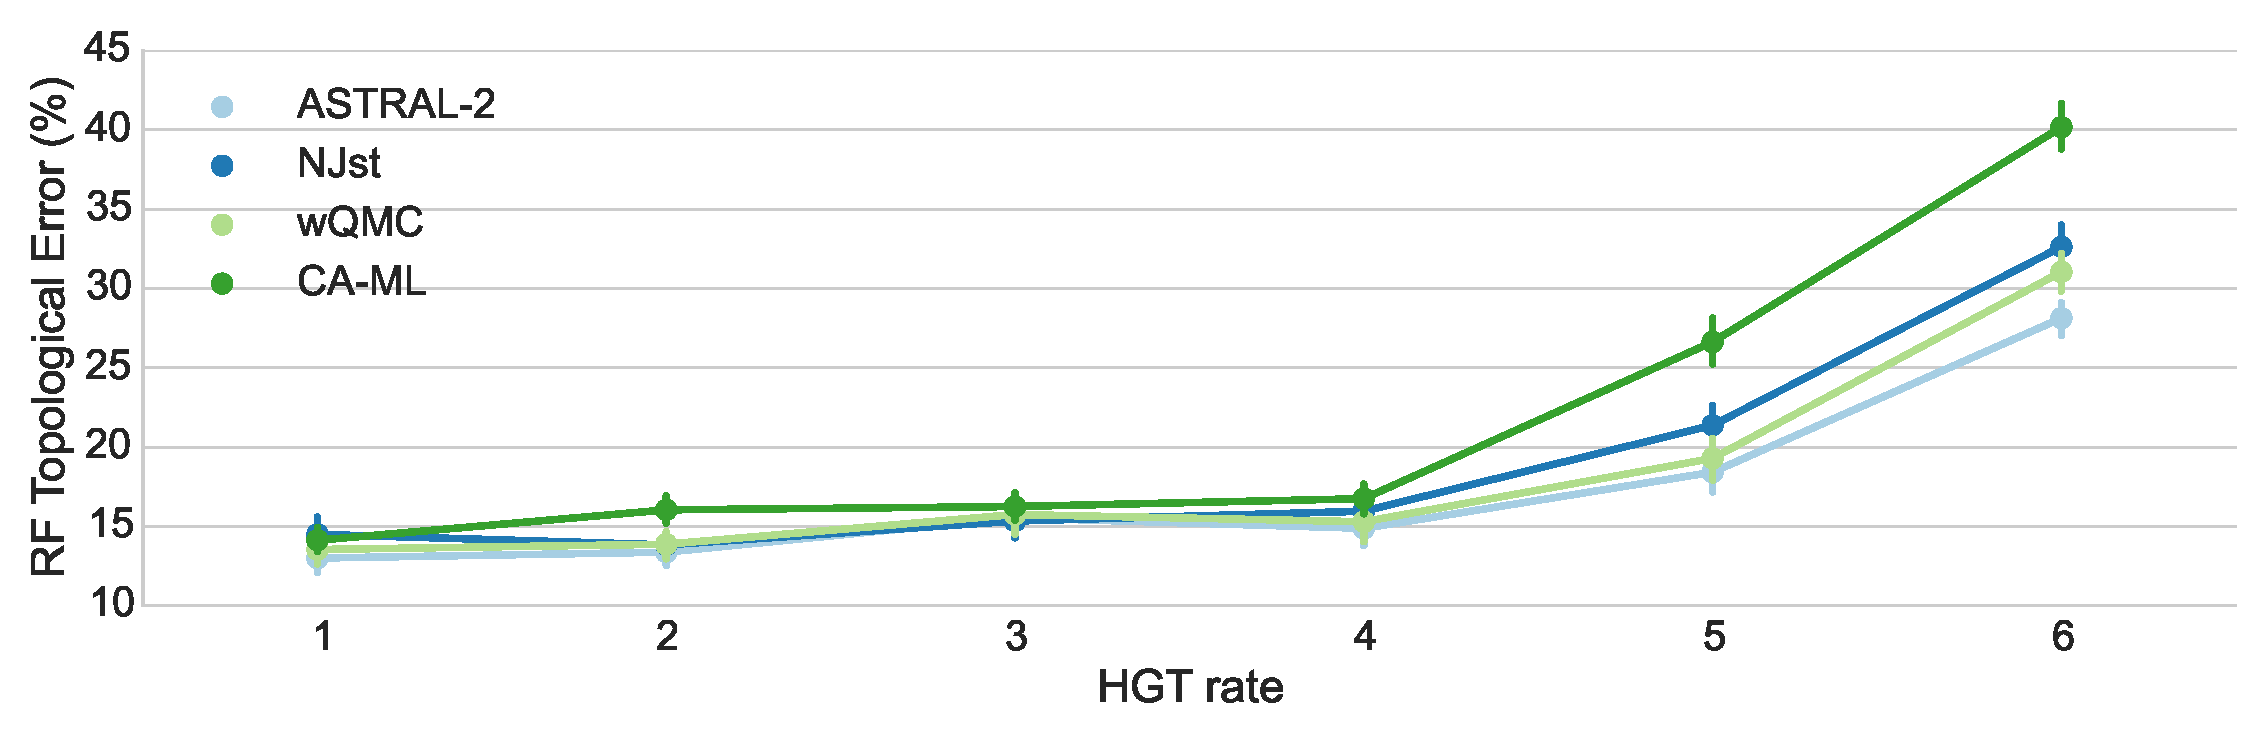
\includegraphics[width=12cm]{hgt-figs/10-est.eps}
 \caption[Mean Robinson-Foulds error rate on 
datasets with 10 genes]{{\bf Mean Robinson-Foulds error rate on 
datasets with 10 genes. } We
show mean RF error rates for summary methods applied to
estimated gene trees as well as for an unpartitioned
maximum likelihood 
concatenation analysis. Error bars indicate standard error; 
50 replicates per dataset. 
}
\label{hgt::fig1}
      \end{figure}

\subsection{Results on estimated gene trees}

For datasets with 10 genes (Fig.~\ref{hgt::fig1}), %
 all the methods are very similar when there is no HGT (i.e., HGT rate (1)), with error rates varying from 13.0\% (ASTRAL-2 and wQMC) to 14.5\% (NJst). Error rates increase with increasing HGT rates, but the increases
are generally small until HGT rate (4), where all methods have error between 14.9\%  (ASTRAL-2) and
16.8\% (CA-ML).   Furthermore,  the differences between methods remain small (no more than 1.9\% between the methods) through HGT rate (4).  However, there are substantial differences between methods under the two highest HGT rates (5) and (6),  with CA-ML having the highest error (26.6\% and 40.2\%, respectively) and ASTRAL-2 having the least error (18.4\% and 28.1\%, respectively). While the differences between wQMC and NJst were often small, typically wQMC was more accurate than NJst. 

%Ruth: fixed figure caption
  \begin{figure}[h!]
 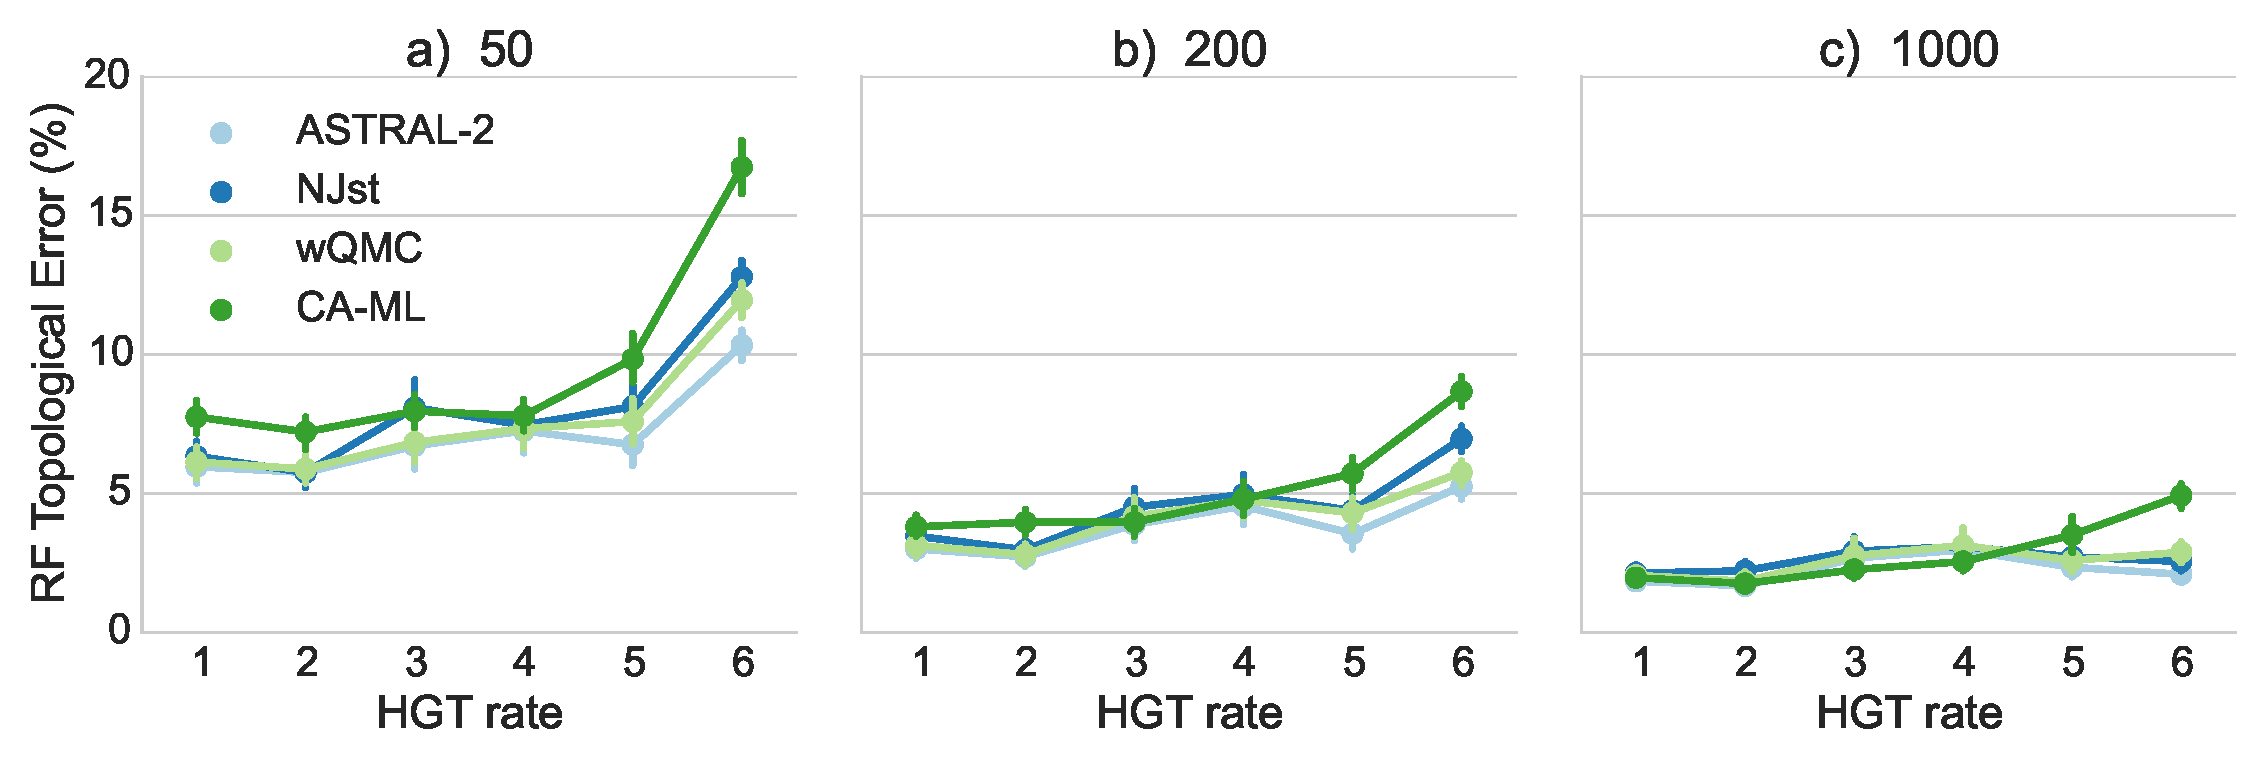
\includegraphics[width=12cm]{hgt-figs/more-est-row.eps}
 \caption[Mean Robinson-Foulds error rates on 
datasets with 50, 200, and 1000 estimated gene trees]{{Mean Robinson-Foulds error rates on 
datasets with 50, 200, and 1000 estimated gene trees. }
We show results for summary methods 
applied to estimated gene trees as well as for an unpartitioned
maximum likelihood
concatenation analysis. Error bars indicate standard error; 
50 replicates per dataset. }
\label{hgt::fig2}
      \end{figure}

The same trends hold on datasets with larger 
numbers of genes (Fig.~\ref{hgt::fig2}); in particular, ASTRAL-2 remains typically the most accurate method (or close to the most accurate method) and CA-ML is typically the least accurate.  However, as the
number of genes increase, the species tree estimation error drops for all methods, and the differences between methods become even  smaller.  For example, on 50 genes the maximum
error for HGT rates (1)-(4) is 7.8\% (CA-ML)  and 
the smallest error is 7.3\% (ASTRAL-2 and NJst). 
By 200 genes, the maximum error of all methods on HGT rates (1)-(4))  is 
5.1\% (NJst) and the smallest is 4.5\% (ASTRAL-2). 
With
1000 genes, the maximum error on HGT rates (1)-(4) is only 3.1\% (wQMC and NJst) and  the lowest is 2.5\% (CA-ML).  
However, under the two higher HGT rates (HGT rates (5) and (6)), the differences between
methods can be noteworthy, even with large numbers of genes. 
More importantly, under these higher HGT rates, 
CA-ML is substantially less accurate than all of the summary methods. 
As an example, under HGT rate (6), 
CA-ML has 16.8\% error on 50 genes, 
while ASTRAL-2 has 10.3\% error. 
One interesting trend that is hard to explain is that error
rates do not always increase with increases in HGT rates; 
for example, results on 1000 estimated trees show some small
 decrease in error
for ASTRAL-2 and NJst between HGT rates (4) and (6). 
Finally, while ASTRAL-2 is the most accurate of the 
summary methods, but
the difference between ASTRAL-2 and the other summary methods is small (ranging from  0.3\% to 1.9\%). 
Indeed, the differences between 
the summary methods given 400 or more genes are very small — 
at most 0.9\%. 


%Ruth: I did not add additional discussion to this part-we told the reviewer we would point out that NJst  yet because we do already address the fact that differences between error rates are small!  I just changed the sentence order so that they could skim and catch the final sentence.  

\subsection{Results on true gene trees}

%We show results for our experiments using ASTRAL, NJst, and wQMC on 10 true gene trees in Figure \ref{hgt::fig3}, and results for these three methods on 50, 200, and 1000 true gene trees in Figure \ref{hgt::fig4}. 
We show results on true gene trees in Figures \ref{hgt::fig5} and
\ref{hgt::fig6}.
  \begin{figure}[h!]
 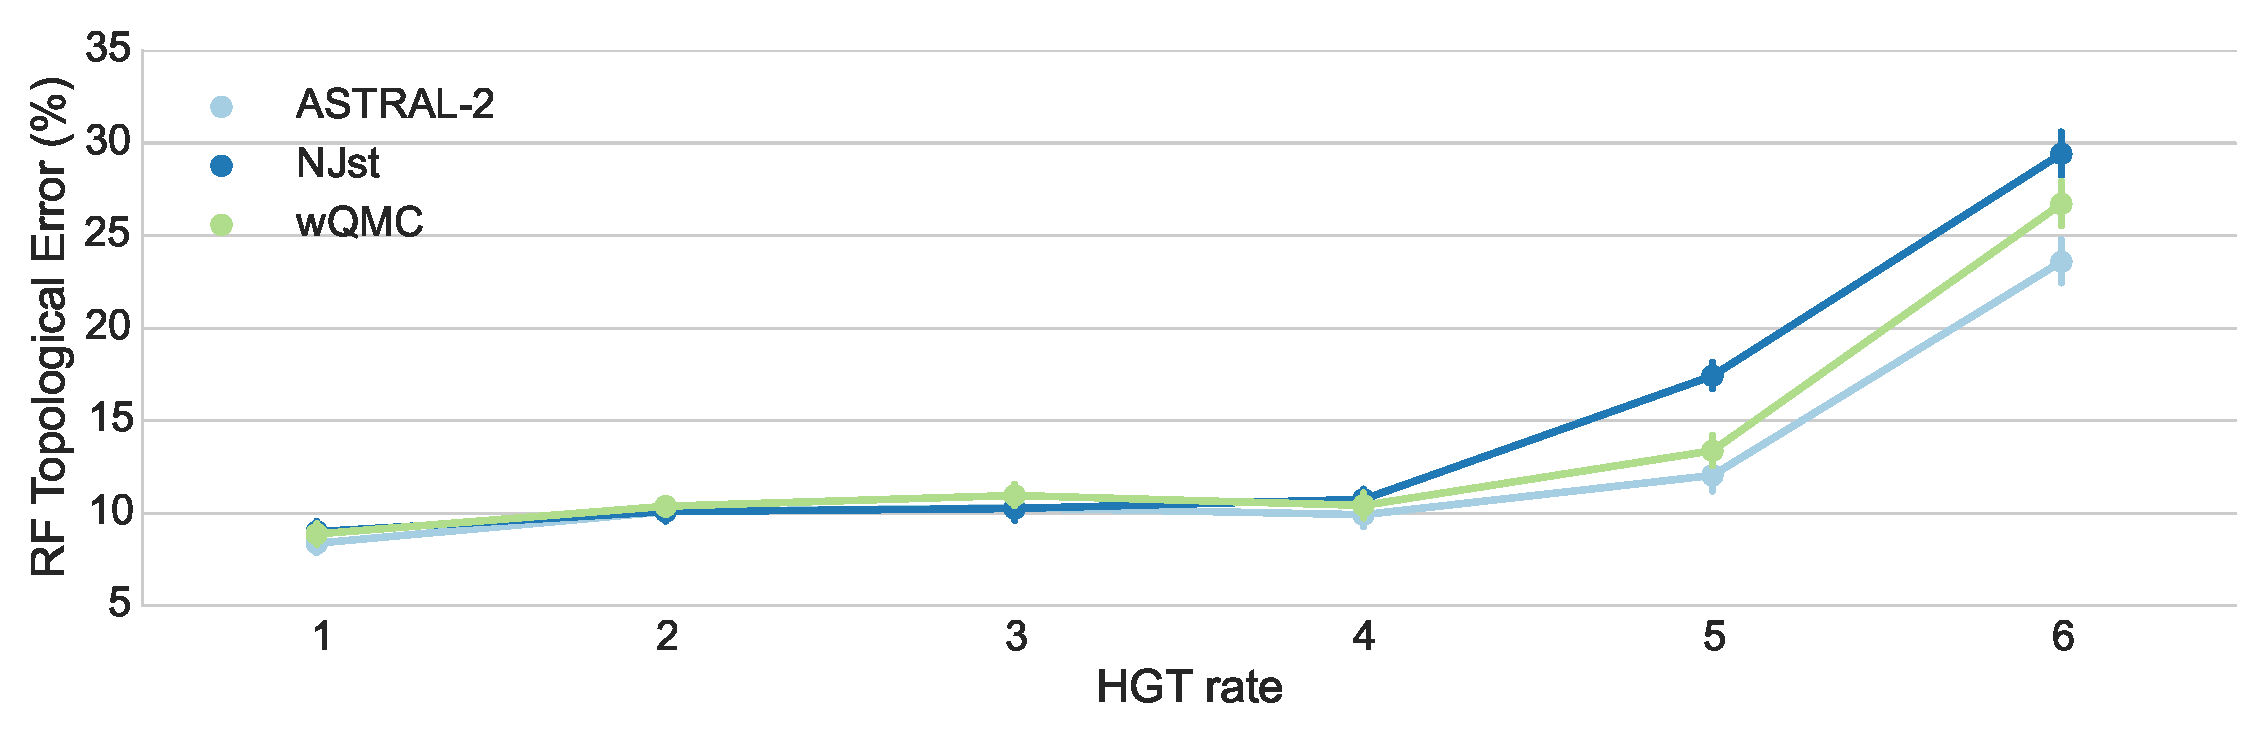
\includegraphics[width=12cm]{hgt-figs/10-true.eps}
 \caption[Mean Robinson-Foulds error rates on 10 true gene trees]{{Mean Robinson-Foulds error rates on 10 true gene trees}. We show
mean RF error rates of summary
methods applied to true gene trees;  error bars indicate standard error. 50
replicates per model condition.}
\label{hgt::fig5}
      \end{figure}
  \begin{figure}[h!]
 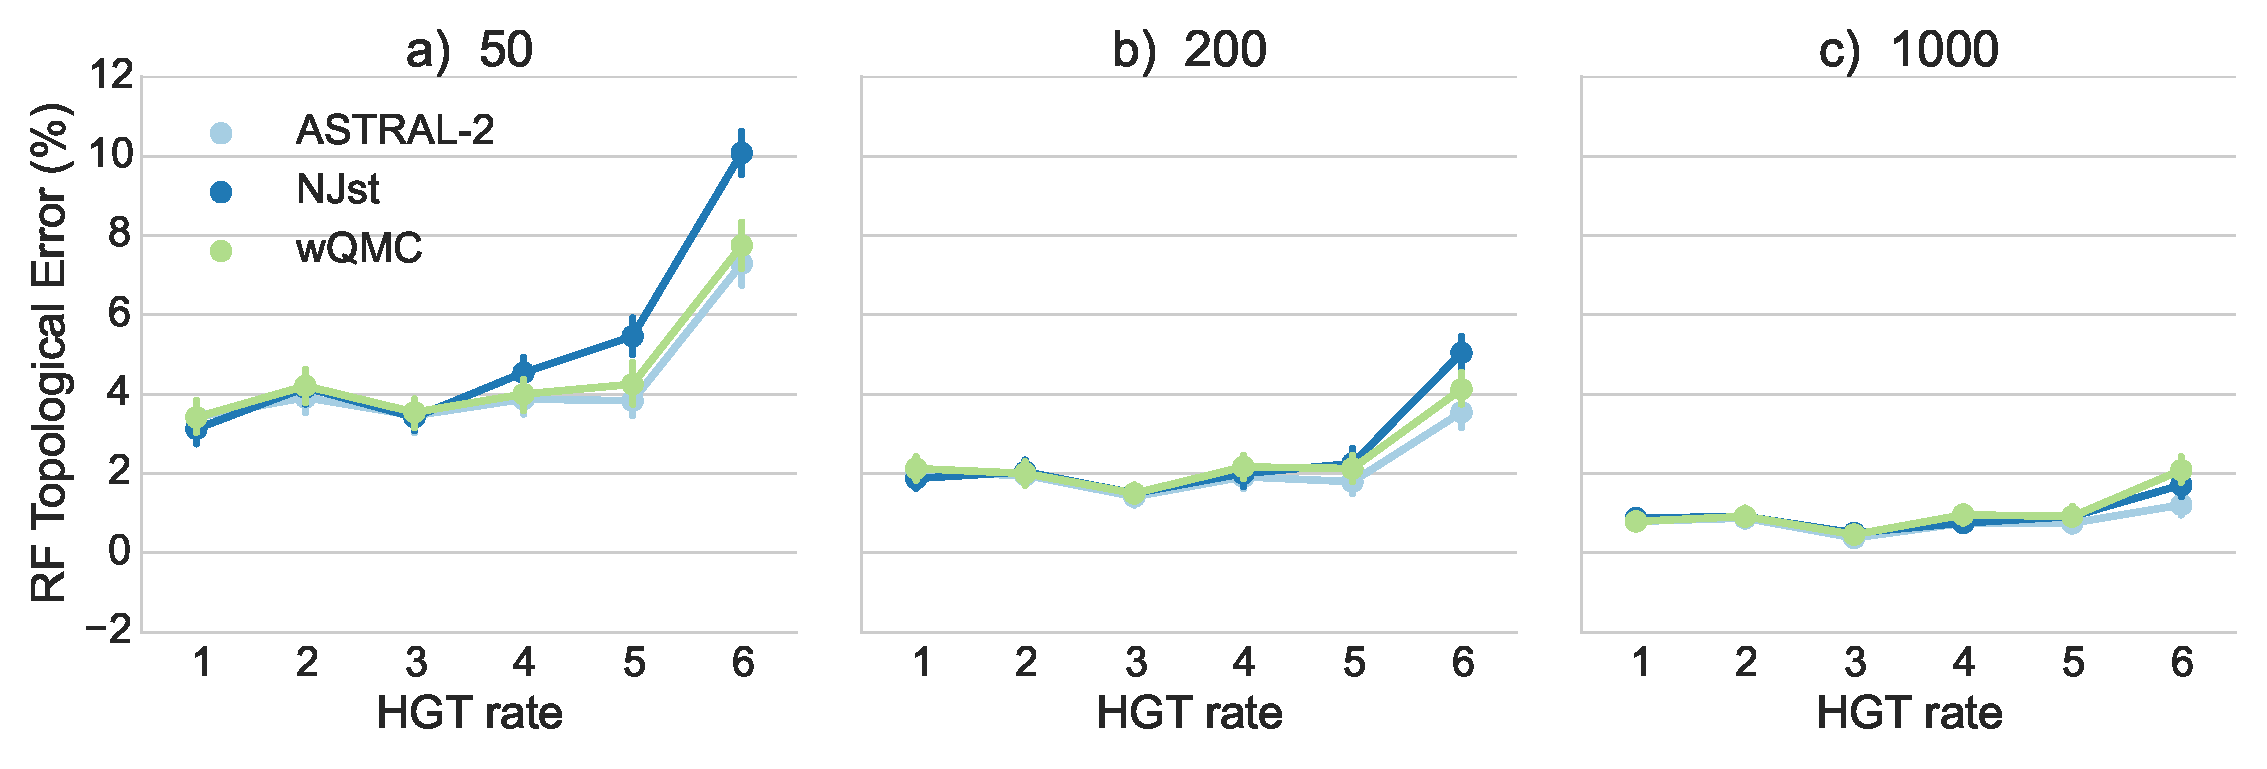
\includegraphics[width=12cm]{hgt-figs/more-true-row.eps}
 \caption[Mean Robinson-Foulds error  rates on 50, 200, 
and 1000 true gene trees]{{Mean Robinson-Foulds error  rates on 50, 200, 
and 1000 true gene trees}. We show
mean RF error rates of summary
methods applied to true gene trees; error bars indicate standard error. 
50 replicates per model condition.}
\label{hgt::fig6}
      \end{figure}
Unsurprisingly, error rates of species trees estimated on true gene trees are lower than those estimated on estimated gene trees;
while the reduction
depended on the model condition,  for the ASTRAL-2 datasets
with 1000 genes and HGT rate (1), we see a reduction of more than 50\%.    
Differences between methods were reduced on the true gene trees, but
otherwise, all the trends are the same as for estimated gene trees.
%As before, ASTRAL-2 was generally the most accurate method. 
%Interestingly, while NJst was rarely as accurate as wQMC method on
%estimated gene trees, given a sufficient number
%of true gene trees NJst was often more accurate than wQMC and sometimes tied with ASTRAL.
%Otherwise, trends observed on the true gene trees
%are generally the same as those observed on estimated gene trees. 
 
\subsection{Comparing quartet scores of trees produced by ASTRAL-2 and wQMC}

While the differences between ASTRAL-2 and wQMC are often
small, ASTRAL-2 nearly always matches or improves on wQMC with respect to tree
topology.  Both ASTRAL-2 and wQMC attempt to 
solve the Maximum Quartet Support Species Tree problem (MQSST, see Methods), but
use very different techniques. In particular,  ASTRAL-2
constrains the search space based on the input gene trees, and
then finds an optimal solution within that constrained space, but
 wQMC uses a greedy
heuristic and does not constrain the search.  
One hypothesis for the improved topological accuracy of ASTRAL-2 compared to wQMC is
that ASTRAL-2 finds better solutions to the MQSST optimization problem, and
a competing hypothesis is that the higher topological
accuracy achieved by ASTRAL-2 is 
due in part 
to the constraint it imposes on the solution space.  




%Table \ref{hgt::table:13} 
%\footnote{Ruth - we need this table. } 
%shows the percentage of times ASTRAL-2 and wQMC find trees with
%the same quartet support score, the percentage of times ASTRAL-2 produces trees with
%better scores, and
%the percentage of times that wQMC produces trees with better scores.  
We examined the quartet scores for  wQMC and ASTRAL-2
across the different model conditions.
% (Table \ref{hgt::table13}).
%
For  57.2\% of all cases involving estimated gene trees, the species trees returned by the two methods had the same quartet support.  ASTRAL-2 returned a tree with a better quartet score than wQMC 29.8\% of the time while wQMC returned a tree with a better quartet score 13.0\% of the time.  
%On true gene trees, ASTRAL-2 has an even bigger advantage over wQMC with
%respect to quartet support scores\footnote{would be good to give numbers. just say (X versus Y).}.%Jun17; see footnote
Thus, in general ASTRAL-2 does a better job than wQMC of finding good solutions to MQSST. 
However, there are cases in which wQMC produces trees with better scores, and the cases
are typically cases with high HGT levels (i.e., there are no cases with HGT rate (1), and  more than half of the cases occurred for HGT rate (6)).  

We investigated the 29 replicates for which wQMC has a better quartet support score, and therefore does a better job of solving the MQSST problem
(Fig.~\ref{hgt::fig5}).
ASTRAL-2 and wQMC had the same topological accuracy on 8 datasets,
ASTRAL-2 was more topologically accurate on 12, and
wQMC was more topologically accurate on 9. 
Thus, even for those cases where wQMC finds trees with better quartet
support scores, ASTRAL-2 
tends to match wQMC with respect to accuracy, or 
produce topologically more accurate trees.
%Thus, optimizing the
%quartet support score is beneficial.
Since wQMC does not constrain the search space, this means
that wQMC can find trees with better quartet scores but which are
outside the constrained search space, and that constraining
the search space seems to be beneficial with respect to
topological accuracy. In other words, 
although ASTRAL-2 generally is a better heuristic for the MQSST
problem, part of the reason it is more topologically accurate
is due to the constraint it imposes on the search space.


  \begin{figure}[h!]
 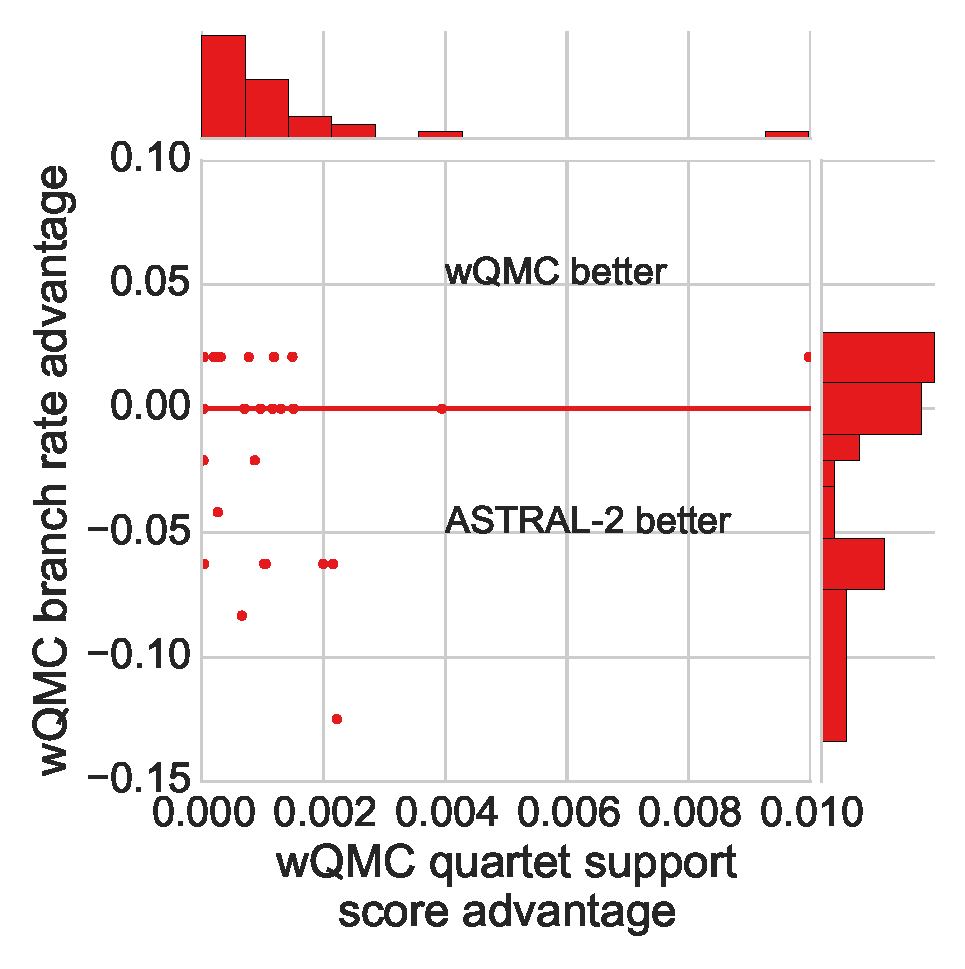
\includegraphics[width=8cm]{hgt-figs/quartet-score-comparison.eps}
 \caption[Differences in quartet support scores
and topological error of wQMC and ASTRAL-2  trees]{{Scatterplot of differences in quartet support scores
and topological error of wQMC and ASTRAL-2  trees. } 
Each point $(x,y)$ represents a dataset in which
wQMC produced a tree with quartet support score 
$x$ points higher than produced by ASTRAL-2, and
with tree topological error $y$ points lower. 
All values of $x$ are strictly positive 
 %Jun17 - see small changes below
(we are only showing cases where wQMC % always
produces a better quartet support score %on these datasets
than ASTRAL-2), but values of $y$ can be arbitrary.
Points with $y < 0$ indicate datasets where ASTRAL-2 produces
a topologically more accurate tree than wQMC, points with $y=0$
indicate datasets where ASTRAL-2 and wQMC produce trees of equal accuracy,
and points with $y>0$ indicate datasets where ASTRAL-2 produces
a tree that is topologically less accurate than wQMC. 
Of the points that are not on the $y=0$ line, more are below
the $y=0$ line than above (i.e., 12 below compared to 9 above), 
indicating that ASTRAL-2 tends to
produce  more accurate tree topologies than wQMC on these datasets.
%ASTRAL has more datasets where it produces a more
%topologically accurate tree than wQMC
%(there are 9 datasets where wQMC has better topological accuracy,
%12 where ASTRAL has better accuracy, and 8 where they they have
%the same accuracy). 
Also, when wQMC is more accurate, the
improvement is lower than when ASTRAL-2 is more accurate.
Thus, even when wQMC finds trees with better quartet scores, ASTRAL-2
tends to produce more topologically accurate trees.
Plots in the margins are histograms of the $x-$ and $y-$axes.
%Most of the replicates for which wQMC has a better 
%quartet score also are the same or better for wQMC in branch rate.  The top half of the main figure plots points for wQMC trees with a lower topological error rate. The right half of the main figure plots points for which wQMC has a better quartet
%score.
} 
\label{hgt::fig4}
       \end{figure}



\subsection{Cyanobacterial Data}

We analyzed a cyanobacterial data set from \cite{Cyanobacteria} using ASTRAL-2 with multi-locus bootstrapping (see Methods) to 
estimate a species tree.   
Two estimated species trees were
reported in \cite{Cyanobacteria}: one is the
``plurality tree", which has served
as the reference tree for this dataset.
The plurality tree is a supertree (computed using
MRP \cite{baum_mrp_2004}) on a set of
quartet trees represented in a plurality of 
the gene trees that have high support. 
The other tree is a PhyML \cite{PhyML} maximum likelihood
tree. 
The ASTRAL-2 majority consensus tree (see Methods) 
has 100\% bootstrap support on all its branches, and is 
identical to the plurality tree; 
that has served as the reference tree for this dataset.
The wQMC tree was previously reported for this dataset in \cite{wQMC}, and is
also topologically  identical to the plurality tree. 
%However, the plurality tree is just a supertree (computed
%using  Matrix Representation with Parsimony \cite{MRP}) on
%the same set of quartet trees that are used by  wQMC. 
%\footnote{Ruth, et al. - we need to find out what exactly the plurality tree 
%is based on, not guess... . }
%Hence, the similarities between these trees are to be expected.  



\section{Discussion}  
While all methods  had very good accuracy on
the simulated datasets under the 
lowest HGT rates, they were clearly differentiated on the higher HGT rates,
especially when the number of genes was not too large. 
Specifically, on the higher HGT rates, concatenation using 
maximum likelihood and NJst were both less
accurate than ASTRAL-2 and wQMC. 
However, all summary methods we explored were impacted
by gene tree estimation error. Furthermore,   there are no proofs
of convergence to the true species tree if the gene
trees have estimation error for these or other
standard summary methods \cite{RochWarnow,WarnowCurrents2015}.
Since many of the lower HGT model conditions
had substantial gene tree heterogeneity resulting from ILS,
this study shows that many methods — and even unpartitioned concatenation  using
maximum likelihood - can be highly accurate under these highly heterogeneous 
model conditions. 

Results on the biological dataset showed that ASTRAL-2 and
wQMC both matched the reference ``plurality tree", and
hence may be correct. But this analysis is perhaps less helpful, since
the reference tree is based on the MRP analysis of a set of quartet
trees, and MRP on quartet trees is a heuristic for the unweighted
version of the optimization problem addressed by wQMC and ASTRAL-2.
Thus, the three methods are closely related in terms of their
optimality criteria, and this may explain why they produce 
the same tree on this input.


This experimental study evaluated the
performance of these methods when HGT is also present, and demonstrated that
wQMC and ASTRAL-2 maintained good accuracy even in the presence of HGT, while NJst tended
to be more impacted by high levels of HGT. 
The explanation as to why NJst is not as robust to high HGT levels as ASTRAL-2 and
wQMC is likely to be that the theoretical justification for NJst only
applies to the MSC model, and not to the
bounded HGT models. 
On the other hand, both ASTRAL-2 and wQMC attempt to solve the 
MQSST problem, for which
optimal solutions are statistically consistent under the MSC model,
and also under the bounded HGT models discussed in \cite{RochSnir}.

Finally, the slight advantage ASTRAL-2 had over wQMC in terms
of topological accuracy is largely due to its
better ability to find good solutions to the MQSST problem, but
constraining the search space is also part of the reason that
ASTRAL-2 has  good topological accuracy, even under conditions
with very high rates of HGT.
%ASTRAL-2 nearly always had quartet support scores that matched or improved on the scores obtained by wQMC, suggesting that improving quartet scores results in improved topological accuracy. On the other hand, ASTRAL-2 constrains the solution space by restricting the species trees it considers to those that draw their bipartitions from a set that ASTRAL-2 computes from the input trees. This constraint on the search space seems to generally not hurt the  search for optimal trees. However, for the few cases where wQMC found better quartet scores, the trees returned by wQMC were 
%generally at least as  topologically accurate as those found by ASTRAL.



\section{Conclusions}
This study evaluated ASTRAL-2, NJst, wQMC, and 
concatenated analysis using unpartitioned maximum likelihood 
(CA-ML) on one 
biological and several simulated datasets in which ILS and HGT were both present.
We observed that the quartet-based methods (ASTRAL-2 and wQMC) generally had
better accuracy than NJst, and that CA-ML could be more accurate than
all methods under conditions with low HGT rates.
In particular, ASTRAL-2, a species tree 
estimation method that was initially 
designed to estimate species trees in the presence of ILS,
had excellent accuracy and generally gave somewhat more accurate
results than the other methods we explored.  However,
all methods were highly accurate under the 
low to moderate HGT levels, and were only differentiated under the two highest HGT levels. 
The methods based on quartets (i.e., wQMC and ASTRAL-2) had the highest robustness to HGT.
While the study is limited in scope, the results suggest that highly accurate species trees can be constructed, even in the presence of both HGT and ILS, using quartet-based methods.

As noted, 
ASTRAL-2 and NJst  are statistically consistent under the MSC model (in which only ILS occurs), and ASTRAL-2 is also statistically consistent
under the bounded HGT models addressed by \cite{RochSnir}. 
However, NJst has not been shown to be statistically consistent 
under the bounded HGT models, and wQMC may not be statistically
consistent under either model (because it is not guaranteed to
solve its optimization problem exactly, 
even when all the dominant quartet trees are compatible).
Because the proof of statistical consistency for ASTRAL-2
depends only on the requirement that for all sets of four
taxa, the most probable quartet tree is
topologically identical to the induced species tree on the four taxa, 
we conjecture that
ASTRAL-2 will be statistically consistent under models in which both ILS and HGT occur but
at bounded rates (where the bounds on one process will depend on the other's bounds).

Although the results in this study are encouraging, 
future work needs to evaluate the performance of species tree
estimation methods under a broader set of conditions. 
In particular, we only evaluated performance under the stochastic HGT model; future work should evaluate methods under the highways model as well.
%Jun17 see addition.
Our datasets had only one level of ILS, and
it is possible that under conditions with higher 
or lower levels of ILS, the effect of HGT would be different. 
This study was limited to gene trees in which heterogeneity was due only to ILS and HGT; future studies should examine other sources of discord, including gene duplication and loss, and/or orthology detection errors. 
Larger numbers of taxa, and/or gene trees with missing taxa, are also likely to present significant analytical challenges, and accurate estimation may not be as easily obtained.
Hence, future studies should also evaluate accuracy on larger
and more challenging
datasets, in order to determine whether the good accuracy
we saw for the quartet-based methods
is maintained under more difficult conditions.
Similarly, it is possible that some methods might provide highly accurate
results on smaller numbers of species, and that the relative
performance of methods could change on those conditions.
Thus, performance on small datasets (with perhaps only 10 species) should
also be explored.

%Ruth: added more text here for additional reviewer response.  I know PHYml was in bib at one point due to longer discussion of cyanobacterial data
This study was limited in terms of the methods that were
explored, in that we restricted the analysis to reasonably
fast methods, and of these fast methods we only explored
those methods
that had been shown to perform well under ILS-only scenarios.
However, it is possible that some coalescent-based species 
tree estimation methods, such as
MP-EST, STAR, etc., might perform
well under HGT+ILS scenarios.
It is also likely  some computationally 
intensive methods, such as BUCKy-pop,
*BEAST, and BEST,  might provide
better accuracy than ASTRAL-2 
on datasets with HGT+ILS. 
There are also methods designed to infer species trees in the presence of
gene tree discordance resulting from duplication and loss, and it is
possible that 
some of these methods (e.g., PhylDog \cite{phyldog} and
MixTreEM \cite{MixTreEM}) might 
have good accuracy under the MSC.
Future work should also explore CA-ML using different ML heuristics
(e.g., PhyML \cite{PhyML}, nhPhyML \cite{nhPhyML}, IQTree \cite{IQTree})
and under more complex sequence evolution models. 
In addition,  it would be very interesting to explore
fully partitioned ML 
analyses, since these have very different statistical properties
than unpartitioned analyses \cite{WarnowCurrents2015}.
% FastTree-2 is a ML heuristic that only allows for unpartitioned maximum likelihood analysis, so additional comparisons are needed using methods such as RAxML  that allow for partitioned analysis, established ML methods such as PhyML \cite{PhyML} as well the newer methods IQTree \cite{IQTree} that has been shown to produce trees with better likelihood scores than RAxML and PhyML under some conditions. 

%Ruth: here is IQTree citataion

%Lam-Tung Nguyen, Heiko A. Schmidt, Arndt von Haeseler and Bui Quang Minh.  IQ-TREE: A Fast and Effective Stochastic Algorithm for Estimating Maximum-Likelihood Phylogenies. Mol Biol Evol (2015) 32 (1): 268-274.


\section{Methods }

\subsection{Species tree estimation methods}
\subsubsection{Maximum Quartet Support Species Tree Problem}

ASTRAL, ASTRAL-2,  and wQMC all address the same optimization problem, 
which we now explain.  Given an input set $\mathcal{G}$ of gene 
trees on a species set $S$ and a quartet tree $q$ on four species from  $S$, 
we let $n(\mathcal{G},q)$ denote the number of gene trees in $\mathcal{G}$ that
induce the quartet tree $q$. Then, the 
\emph{quartet support} of $T$ given $\mathcal{G}$, denoted $w_{\mathcal{G}}(T)$, is 
$\sum_{q \in Q(T)} n(\mathcal{G},q)$, where $Q(T)$ denotes the set of all quartet
trees in $T$.
Hence, we can define the {\em Maximum Quartet Support
Species Tree Problem} (MQSST),  as follows. 


\begin{itemize} 

\item Input: a set of gene trees $\mathcal{G}$ on a species set $S$. 

\item Output: a tree $T$  on the species set $S$ maximizing 
$w_{\mathcal{G}}(T)$, 
the quartet support of $T$ given $\mathcal{G}$.

\end{itemize}
\noindent
MQSST is $NP$-hard when the input 
 %Jun17 - see change below
 set of gene trees induce only one tree for each set of four taxa in $S$ 
 \cite{JiangPTAS}, and is of unknown
computational complexity when all the gene trees are complete
(i.e., have all the species in $S$).

\subsubsection{Weighted Quartets MaxCut}
The quartet amalgamation method 
wQMC \cite{wQMC} is 
%Quartets Max Cut
%(QMC) \cite{QMC},   which is 
a greedy heuristic for 
a weighted version of 
the MQSST problem, 
%The difference
%between wQMC and QMC is that
in which 
the input can have
weights on each quartet tree.
The
wQMC heuristic uses a greedy strategy to
find good solutions to its
optimization problems, but is not guaranteed to solve its
optimization problem (weighted MQSST) exactly. 
To use wQMC as a summary method, 
we define the weight of a quartet  tree $q$ to be 
the quartet support $n(\mathcal{G},q)$ of $q$ 
in the input set of gene trees $\mathcal{G}$. 
%We chose wQMC as a method to use in this paper because QMC is a fast heuristic when the number of input quartets is reasonably small; the number of weighted quartets input to wQMC used as a summary method  is $O(n^{4})$, so we can run wQMC as a summary method on moderately sized sets of taxa such as our 51-taxon simulated data sets. 
%using a script based on code from \cite{JohansenThesis} summarized in a file
%
%\noindent \begin{verbatim} <quartetfilename> \end{verbatim} 
%
%\noindent and used this frequency as a weight for the quartet. The command used was 
 
 
%  \begin{verbatim} cat <quartetfilename> | sed s/"(("//g | sed s/"),  \end{verbatim} \begin{verbatim} ("/"|"/g | sed s/")); "/":"/g | \end{verbatim} \begin{verbatim} sed '/|/!d' >  <fixedfilename> \end{verbatim} \begin{verbatim} ./max-cut-tree qrtt=<fixedfilename> \end{verbatim} \begin{verbatim} sed '/|/!d' >  <fixedfilename> \end{verbatim} \begin{verbatim} weights=on otre=<treefilename> \end{verbatim}  
%We used wQMC version  3.0,
%using the following command:
%\begin{verbatim}
%sh quartet_count.sh <genetrees> | perl summarize_quartets_stdin.pl  
%\end{verbatim}
%\begin{verbatim}
%| sed s/"(("//g | sed s/"),("/"|"/g | sed s/")); 
%\end{verbatim}
%\begin{verbatim}
%"/":"/g | sed '/|/!d' > <quartetscores>
%./max-cut-tree qrtt=<quartetscores> weights=on otre=<speciestree>
%\end{verbatim}

 %Jun17 - changed this part
We wrote scripts (available in our supporting online  material)
that use a previously published code~\cite{JohansenThesis}
to compute the weights of each quartet tree.
After we calculate these weights (saving them in a 
file called {\tt <quartetscores>}),
we run wQMC version 3.0 using the following command:
\begin{verbatim}
./max-cut-tree qrtt=<quartetscores> weights=on otre=<speciestree>
\end{verbatim}

\subsubsection{ASTRAL and ASTRAL-2}
ASTRAL \cite{Astral} and 
its improved version, 
ASTRAL-2 \cite{Astral2}, 
also attempt to solve the MQSST problem.
Both have exact versions that provably solve the
MQSST problem but run in exponential time, and faster
versions that constrain the search space (using the input
set of gene trees), and then provably solve the
constrained problem exactly.
ASTRAL and ASTRAL-2 differ in
how they constrain the search space (ASTRAL-2 searches
a larger part of tree space than ASTRAL)  and how
they are implemented (ASTRAL-2 is faster). 
Here we focus on ASTRAL-2, since it is faster
and more accurate than ASTRAL. 

Given
the input set of gene trees, ASTRAL-2 defines a set $\mathcal{X}$ of
bipartitions on the taxon set $S$; when all the gene trees are
complete (i.e., have no missing taxa), then $\mathcal{X}$ will 
contain all the bipartitions from the input gene trees as well as potentially
other
bipartitions.
ASTRAL-2 runs in $O(n k |\mathcal{X}|^2)$ time, where
$n$ is the number of species and $k$ is the number of genes, and thus
can be fast whenever $|\mathcal{X}|$ is not too large.
While $|\mathcal{X}|$ is not theoretically bounded by
a polynomial in $n$ and $k$, 
for many datasets $|\mathcal{X}|$ is
not very large, so that
ASTRAL-2 is able to complete analyses 
within 24 hours  on 
1000 species and 1000 genes \cite{Astral2}.

ASTRAL-2
finds a globally optimal solution to the constrained optimization problem
where we restrict the output species tree to draw its bipartitions
from $\mathcal{X}$. 
ASTRAL and ASTRAL-2, run in their default versions (which
use the constrained search),  are both
statistically consistent under the multispecies
coalescent model when all the gene trees are complete (i.e.,  this restriction
to the set $\mathcal{X}$ of bipartitions does not change
their statistical guarantees) \cite{Astral2}.

We now provide a proof for  Theorem \ref{hgt::theorem-corollary}, establishing that
ASTRAL and ASTRAL-2, 
run in default mode,
are statistically consistent under the MSC model and also 
under the bounded
HGT models. 

%Ruth: removed sketch comment, added a few words here are there
\noindent
{\bf Proof for Theorem \ref{hgt::theorem-corollary}}.
As proved in \cite{Astral,Astral2}, 
 ASTRAL and ASTRAL-2 are guaranteed to
find globally optimal solutions to the constrained MQSST problem. 
The default settings for the constraint set $\mathcal{X}$ of
bipartitions allowed in the output species tree always includes all bipartitions from the input
gene trees; hence, as the number of genes increases, 
with probability converging to $1$, every
bipartition from the species tree will be in the set $\mathcal{X}$.
Therefore, with probability converging to $1$, the true
species tree will be a feasible solution (i.e., within the
constrained search space) as the number of loci
and number of sites per locus both increase (as established
in \cite{Astral,Astral2}). 
Recall that the quartet support score of a tree
$T$
is 
%Then, given a set of quartet trees for which the dominant
%quartet trees are identical to the species trees, the 
%true species tree will have a higher
%quartet support score than for any other tree;
%this follows by observing that the quartet support score of a tree $T$ is
the total, over all quartet trees in $T$, of the number of
gene trees that contain that quartet tree. % and that the dominant
%$T$
%quartet tree appears more often than the alternative quartet trees.
%As has already been established, there are no anomalous
%four-leaf trees, and hence
%under the MSC model 
As shown in \cite{RochSnir}, 
under the bounded HGT models in \cite{RochSnir},
the most
probable quartet tree on any four taxon set  $A$ is topologically 
identical to the quartet tree on $X$ induced by the
true species tree.
Hence, 
with probability 
converging to $1$, under these
bounded HGT models, the most
frequent quartet tree on any set $A$ of 
four leaves will be the true species tree on $A$.
Given any set of gene trees
in which for all four-leaf sets $A$ the most frequent quartet
tree on $A$ is the true species tree on $A$,
  the quartet support score 
of the true species tree $T^*$ will be
the maximum possible quartet support score (since
any other species tree $T$ cannot have larger
quartet support for any quartet tree).
Furthermore, given any set of gene trees
in which the most frequent quartet tree is
unique for all four taxa and equal to the species
tree on the four taxa, the true species tree $T^*$ will
have the unique maximum quartet support score.
Hence,
as the number of loci and number of sites per locus both increase,
the tree returned by an exact solution to the constrained MQSST
problem, using default settings for $\mathcal{X}$,
will converge in probability to the true species tree $T^*$.
Therefore, ASTRAL and ASTRAL-2 are statistically consistent
under the bounded HGT models of \cite{RochSnir}.

% however, the statistical
%consistency of these methods under models with
%both HGT and ILS is unknown. 
%However, just as it is not clear if other
%quartet amalgamation methods (e.g., QMC and QFM) are statistically
%consistent under the MSC model,
%it is not clear if QMC is statistically
%consistent under these bounded HGT models.

We ran ASTRAL-2 version 4.7.6 on the simulated data using the
following  command:
\begin{verbatim}
java -jar  astral.4.7.6.jar -i <genetrees> -o <speciestree>
\end{verbatim} 
\noindent
where {\tt <genetrees>}  is a file containing 
the gene trees in newick format, and 
{\tt <speciestree>} is the output.




For  the biological data, we used ASTRAL-2 with 
multi-locus bootstrapping (MLBS), using the following commands:
\begin{verbatim}
 java -jar astral.4.7.6.jar -i < bootstrap replicates >  \end{verbatim}
 \begin{verbatim} -o <species replicate> \end{verbatim}
where 
{\tt bootstrap replicates}
is the collection of 1128 gene trees generated by taking the $n^{th}$ line of the gene tree file $n = \{1, \ldots , 100\}$, and
{\tt species replicate}
is the $n^{th}$ bootstrap replicate species tree $T_{n}$.  To calculate the final species tree $T$ with bootstrap support values, we computed the majority consensus tree using Dendropy version 3.12.2  \cite{Dendropy}.  
%This was done by populating a Dendropy TreeList object from the collection $S_{n}$ and then obtaining $T$  via the command 
%\begin{verbatim}  T= dendropy.TreeList.get_from_path(**kwargs) \end{verbatim} and then calling the method \begin{verbatim} Tn.consensus() \end{verbatim} in default mode, which requires the minimum frequency of a split appearing in the consensus tree to be 50\%.
%Ruth - this detail should go into some external document that
%is put on the webpage

\subsubsection{NJst}
NJst is a summary method that 
has two steps. In the first step, it computes a distance matrix on
the species set, where $D[x,y]$ is the average
leaf-to-leaf topological distance between $x$ and $y$ among all the
gene trees. In the second step, it runs neighbor joining \cite{NJ}, a popular
distance-based phylogeny estimation method. 
NJst is statistically consistent under the 
MSC model
because the distance matrix it computes converges in
probability to an additive matrix defining the true
species tree, and neighbor joining will return
the true species tree once the computed distance matrix  is
sufficiently close to the additive matrix for the species tree; see
\cite{njst} for this proof.

 %Jun17 - changed below
To run NJst, we used phybase version 1.4 \cite{phybase}
and custom scripts, available in our supplementary material. 
%{\tt https://faculty.franklin.uga.edu/lliu/content/phybase}, 
%using the following
%command:
%\begin{verbatim}
%./njst <genetrees> <speciestree>
%\end{verbatim}


\subsection{Gene tree estimation}
To compute gene trees, we ran FastTree-2  version 2.1.4, using the following command:
\begin{verbatim}
fasttree -nt -gtr -quiet -nopr -gamma -n 1000 [input] > [output]
\end{verbatim}
where {\tt [input]} is a file that includes all the alignments of all 1000 genes and 
{\tt [output]} will be one file with all 1000 estimated gene trees. 

\subsection{CA-ML}
To perform the concatenated  analyses under maximum likelihood,
we ran FastTree-2 version 2.1.4, with the following
command:
\begin{verbatim}
fasttree -nt -gtr  -nopr  [input] > [output]
\end{verbatim}


\subsection{Computing Error Rates}
The coalescent-based methods ASTRAL-2, wQMC, and NJst used in this study all return binary species trees.   We also verified that all trees returned in our CA-ML analysis were binary, and all simulated data used in this study contained only binary model species trees.  The Robinson-Foulds (RF)  distance \cite{RF} between two trees $T_{1}$ and $T_{2}$ on the same set of  $n$ taxa measures the number of bipartitions that appear in only one of $T_{1}$  or $T_{2}$.  Therefore, if $T_{1}$ and $T_{2}$ are identical, the RF distance is 0, and the maximum RF distance between $T_{1}$ and $T_{2}$ is $2n-6$.  The RF distance can be converted to an error rate by dividing by $2n-6$.   When comparing only binary trees, false negative rates, false positive rates, and normalized Robinson-Foulds distances  are all equivalent.  Therefore, we computed missing branch rates to establish error rates, but we report RF rates. Error rates were computed by finding the missing branch rate using custom scripts available in our supporting online materials.  



\subsection{Measuring Quartet Support Scores of ASTRAL-2 and wQMC}

\noindent The command used to measure the quartet support score was

 \begin{verbatim} java -jar astral.4.7.6.jar -q  <speciestreefile> -i  <genetreesfile>   \end{verbatim}



\subsection{Data}

\paragraph{HGT+ILS Simulated Data}

The simulated dataset was simulated using SimPhy \cite{SimPhy} version 1.0
(downloaded January 20, 2015).   There are 6 data sets containing 50 replicates apiece: each replicate has its own 51-taxon species tree.  For every model species tree, one taxon is an outgroup, and so is actually a 50-taxon rooted species tree.  These model trees were simulated under a Yule process, with birth rates set to $0.000001$ (per generation) and the maximum tree length set to 2 million generations.  

%Tandy - fix next paragraph (after "rate of HGT")
Then, on each species tree, 
1000 locus trees are simulated, where each can differ from the species tree due to HGT events, and we used HGT rates (1)-(6) given by
$0, 2 \times 10^{-9}, 5 \times 10^{-9}$, $2 \times 10^{-8}$, $2 \times 10^{-7}$, and $5 \times 10^{-7}$.  These values correspond to expected numbers of HGT events per gene of 0, 0.08, 0.2, 0.8, 8, and 20. Thus, 
HGT rate (1) is no  HGT  events, 
HGT rate (2) is 0.08 HGT events per gene, up to HGT rate (6) of 20
HGT events per gene. 
%Jun17 - see addition below. 
Note that in our simulations, 
for each HGT event, the probability of a branch being chosen as the 
receptor of the transfer is proportional to its distance from the donor. 
%\footnote{ Ruth, Pranjal, Siavash, -- which of these HGT rates are
%low enough that they fit in the bounded HGT models of Roch and Snir, or
%Steel et al? Also, is the way that we generated the data
%under the same model as the bounded HGT models? In other words,
%check that the bounded HGT models have HGT events that depend on
%the distance between the lineages involved, and check also 
%whether the model for generating the data does the same thing. It may
%not. If not, then we need to specify that we generated the data
%under a different model. The equiprobable model may be easier or
%harder to work with, but we need to discuss this.}

Once locus trees are simulated, a gene tree is simulated for each locus tree according to the MSC model,  with population size parameter set to 200,000.  Thus, at the end, we have 1000 true genes that differ from the species tree due to both ILS and also potentially HGT (when the HGT rate is positive).

The SimPhy command used to generate a model replicate in the data sets is%\footnote{Ruth- some of the parameters are fixed in the experiment
%we ran, as you note below. So why not just substitute
%the fixed values in the command?}
 %Jun17 - check to see if this modified version looks fine in pdf
\begin{verbatim}
simphy -rs 50 -rl U:1000,1000 -rg 1 -st U:2000000,2000000 -si U:1,1 
-sl U:50,50 -sb U:0.000001,0.000001 -cp U:200000,2000000 
-hs L:1.5,1 -hl L:1.2,1 -hg l:1.4,1 -cu E:10000000  -so U:1,1 -od 1 
-or 0 -v 3 -cs 293745 -o model.50.2000000.0.000001.<transferrate>  
-lt U:<transferrate>,<transferrate> -lk 1
 \end{verbatim}
 

%\footnote{Siavash, Ruth, or Pranjal - can 
%you figure suggest a nicer way to format this section?} 
% \begin{verbatim}<replicates>, <treelength>, <numgenes>, <birthrate> \end{verbatim} and \begin{verbatim} <population> \end{verbatim} 
%\noindent
%were fixed at 
%50, 
%2 million, 
%1000, 
%$1e-06$, and 200,000, respectively. To vary HGT rates,  \begin{verbatim}  <transferrate> \end{verbatim} varied across as described above to produce the HGT rates (1)-(6) that are described above. 

%were fixed at 50, 2 million, 1000, $1e-06$, and 200,000, respectively.  

 
On each simulated true gene tree, we used INDELible
 \cite{Indelible} v.~1.03  to simulate sequence alignments according to the GTR+$\Gamma$ model,  with model parameters estimated from three different real datasets (these parameters are identical to those 
used in \cite{Astral2}). 
This simulation  produces 
GTR parameters that vary from one gene to another,
where the parameters are drawn for each gene from a distribution at random. 
%These distributions were Dirichlet (36 26 28 32) for base frequencies and 
%Dirichlet (16   3   5   5   6  15) for the $4 \times 4$
%substitution matrix. The alpha parameter for rates-across-sites 
%was drawn from  an exponential(1.2) distribution, truncated from below at $0.1$. 
%The parameter for these models were estimated from real data. 
See \cite{Astral2} for details about the simulation process.
%INDELible runs using control files always labeled ``control.txt", 
%which are far too large to represent in a manuscript of this type. 
%The control files used to generate the sequence alignments for this data are available in compressed form at  
%\begin{verbatim} https://www.dropbox.com/s/3z1ysh1rq2a7zns/
%\end{verbatim}\begin{verbatim}control-txt-Indelible-controls-for-Davidsonetal.zip?dl=0
%\end{verbatim}
The alignment length is set to 1000bp for all genes. 
After simulating gene alignments, we used FastTree-2 \cite{FastTree2} to estimate gene trees under the GTR model.  Thus for each replicate, we have both true and estimated gene trees.  

For HGT rate (1) (where all the discordance is due to ILS), 
the average RF \cite{RF} distance between 
true gene trees and the species tree is 30.4\%.  
Therefore, the amount of ILS in these data sets is moderately high. 




\paragraph{Cyanobacterial Data}\label{hgt::}

The cyanobacterial data set has
1128 genes on 11 taxa, and was first analyzed in \cite{Cyanobacteria}, which 
suggested that the 11 genome sequences may 
have acquired between 9.5\% and 16.6\% of their genes through HGT.  
We obtained 100 bootstrap replicate gene trees
for each of the 1128 genes from the first author of \cite{BansalHGTProkaryotes}, and computed
an ASTRAL-2 tree on these data using multi-locus bootstrapping.



\section{Tables}

Tables show the results of the 28 experiments we ran on the simulated data set. Rows are labeled by the number of genes input to each experiment, and columns are labeled by the method run on the input set of genes.  Entries in the table are the mean error rate over all 50 replicates analyzed in each experiment, given as a percentage of branches is the model species tree 
missing in the estimated species tree. 
%Since both model trees and estimated trees in our simulated data sets are binary, this is equivalent to the RF distance.  
For all numbers of genes and all HGT rates, the number of taxa in the input gene trees, model species tree, and estimated species tree are fixed at 51. 

Tables (1)-(6) show error rates on estimated gene trees, which include CA-ML results for some numbers of genes. Tables (7)-(12) show error rates on true gene trees.  Both Tables (1)-(6) showing results for estimated gene trees and Tables (7)-(12) showing results for true gene trees are labeled by increasing HGT rate. In all tables, the lowest error rate returned by a method in each row is in bold text.  



\begin{table}[h!]
\caption[error rates of estimated species trees (50 replicates)  on estimated gene trees for HGT rate 1]{Average Robinson-Foulds error rates of estimated species trees (50 replicates)  on estimated gene trees for HGT rate (1): 51 taxa, 1000 bp true alignments}
\begin{tabular}{rrrrrr}
 & Number of Genes & ASTRAL & wQMC  & NJst & CA-ML\\
\hline
 & 10 & \textbf{13.0} & \textbf{13.0} &   14.5 & 14.1 \\
 & 25 & \textbf{8.6} & \textbf{8.6} &   9.5 & \\
 & 50 & \textbf{6.0} & \textbf{6.0} &   6.6 & 7.8 \\
 & 100 & \textbf{4.5} & \textbf{4.5}   & 4.6 & \\
 & 200 & \textbf{3.0} & 3.2 &   3.6 & 3.8\\
 & 400 & \textbf{2.4} & 2.6 &   2.7 & \\
 & 1000 & \textbf{1.8} & 2.0   & 2.1 & 2.0 \\
\end{tabular}
\label{hgt::table1}
\end{table}


\begin{table}[h!]
\caption[Error rates of estimated species trees (50 replicates)  on estimated gene trees for HGT rate 2]{Average Robinson-Foulds error rates of estimated species trees (50 replicates)  on estimated gene trees for HGT rate (2): 51 taxa, 1000 bp true alignments}
\begin{tabular}{rrrrrr}
 & Number of Genes & ASTRAL & wQMC   & NJst & CA-ML\\
\hline
 & 10 & \textbf{13.4} & 13.5 &   13.7 & 16.0 \\
 & 25 & \textbf{8.5} & 8.8 &  8.7 & \\
 & 50 & \textbf{5.7} & 5.9 & 5.8 & 7.2\\
 & 100 & \textbf{3.4} & 3.5  & 4.0 & \\
 & 200 & \textbf{2.7} & 2.8   & 3.1 & 4.0\\
 & 400 & \textbf{2.1} & 2.2   & 2.3 & \\
 & 1000 & \textbf{1.7} & 1.8   & 2.2 & \textbf{1.7} \\
\end{tabular}
\label{hgt::table2}
\end{table}

\begin{table}[h!]
\caption[Error rates of estimated species trees (50 replicates)  on estimated gene trees for HGT rate 3]{Average Robinson-Foulds error rates of estimated species trees (50 replicates)  on estimated gene trees for HGT rate (3): 51 taxa, 1000 bp true alignments}
\begin{tabular}{rrrrrr}
 & Number of Genes & ASTRAL & wQMC   & NJst  & CA-ML\\
\hline
 & 10 & \textbf{15.5} & \textbf{15.5} &   15.6 & 16.3\\
 & 25 & \textbf{9.0} & 9.1 &  9.9 & \\
 & 50 & \textbf{6.7} & 7.0  & 8.0 & 8.0 \\
 & 100 & \textbf{4.9} & 5.3   & 5.6 & \\
 & 200 & \textbf{3.9} & 4.2   & 4.4 & 4.0 \\
 & 400 & \textbf{3.1} & 3.2   & 3.5 & \\
 & 1000 & 2.7 & 2.8 &   3.0 & \textbf{2.2} \\
\end{tabular}
\label{hgt::table3}
\end{table}

\begin{table}[h!]
\caption[Error rates of estimated species trees (50 replicates)  on estimated gene trees for HGT rate 4]{Average Robinson-Foulds error rates of estimated species trees (50 replicates)  on estimated gene trees for HGT rate (4): 51 taxa, 1000 bp true alignments}
\begin{tabular}{rrrrrr}
 & Number of Genes & ASTRAL & wQMC   & NJst & CA-ML \\
\hline
 & 10 & \textbf{14.9} & 15.2 &   15.7 & 16.8\\
 & 25 & \textbf{9.3} & 9.6 &  10.2 & \\
 & 50 & \textbf{7.3} & 7.5  & \textbf{7.3} & 7.8\\
 & 100 & 5.8 & 5.8 &   \textbf{5.5} & \\
 & 200 & \textbf{4.5} & 4.7   & 5.1 & 4.8 \\
 & 400 & \textbf{3.5} & 3.7  & 3.9 & \\
 & 1000 & 3.0 & 3.1 &  3.1 & \textbf{2.5} \\
\end{tabular}
\label{hgt::table4}
\end{table}

\begin{table}[h!]
\caption[Error rates of estimated species trees (50 replicates)  on estimated gene trees for HGT rate 5]{Average Robinson-Foulds error rates of estimated species trees (50 replicates)  on estimated gene trees for HGT rate (5): 51 taxa, 1000 bp true alignments}
\begin{tabular}{rrrrrr}
 & Number of Genes & ASTRAL & wQMC   & NJst & CA-ML\\
\hline
 & 10 & \textbf{18.4} & 19.7 &   21.6 & 26.6 \\
 & 25 & \textbf{10.7} & 11.5   & 12.5 & \\
 & 50 & \textbf{6.8} & 7.6 &  8.3 & 10.0\\
 & 100 & \textbf{5.2} & 5.9 &   6.5 & \\
 & 200 & \textbf{3.5} & 4.3 &   4.2 & 5.7 \\
 & 400 & \textbf{3.2} & 3.8 &   3.6 & \\
 & 1000 & \textbf{2.3} & 2.6   & 2.7 & 3.5 \\
\end{tabular}
\label{hgt::table5}
\end{table}

\begin{table}[h!]
\caption[Error rates of estimated species trees (50 replicates)  on estimated gene trees for HGT rate 6]{Average Robinson-Foulds error rates of estimated species trees (50 replicates)  on estimated gene trees for HGT rate (6): 51 taxa, 1000 bp true alignments}
\begin{tabular}{rrrrrr}
 & Number of Genes & ASTRAL & wQMC  & NJst & CA-ML\\
\hline
 & 10 & \textbf{28.1} & 31.8 &   32.1 & 40.2 \\
 & 25 & \textbf{15.7} & 17.3 &   19.3 & \\
 & 50 & \textbf{10.3} & 11.7 &   13.0 & 16.8\\
 & 100 & \textbf{7.3} & 8.5 &   9.0 & \\
 & 200 & \textbf{5.2} & 6.1 &   7.1 & 8.7 \\
 & 400 & \textbf{3.5} & 4.4 &   4.0 & \\
 & 1000 & \textbf{2.1} & 3.2  & 2.5 & 5.0\\
\end{tabular}
\label{hgt::table6}
\end{table}



\begin{table}[h!]
\caption[Error rates of estimated species trees (50 replicates)  on true gene trees for HGT rate 1]{Average Robinson-Foulds error rates of estimated species trees (50 replicates)  on true gene trees for HGT rate (1): 51 taxa, 1000 bp true alignments}
\begin{tabular}{rrrrrr}
 & Number of Genes & ASTRAL & wQMC &  & NJst\\
\hline
 & 10 & \textbf{8.4} & 8.7 &  & 9.1\\
 & 25 & \textbf{5.0} & 5.2 &  & 5.5\\
 & 50 & 3.4 & 3.4 &  & \textbf{3.2} \\
 & 100 & \textbf{2.5} & 2.6 &  & \textbf{2.5} \\
 & 200 & 2.0 & 2.2 &  & \textbf{1.9}\\
 & 400 & \textbf{1.4} & 1.5 &  & \textbf{1.4} \\
 & 1000 & \textbf{0.8} & \textbf{0.8} &  & 0.9\\
\end{tabular}
\label{hgt::table7}
\end{table}

\begin{table}[h!]
\caption[Error rates of estimated species trees (50 replicates)  on true gene trees for HGT rate 2]{Average Robinson-Foulds error rates of estimated species trees (50 replicates)  on true gene trees for HGT rate (2): 51 taxa, 1000 bp true alignments}
\begin{tabular}{rrrrr}
 & Number of Genes & ASTRAL & wQMC   & NJst\\
\hline
 & 10 & \textbf{10.1} & 10.3 &   \textbf{10.1}\\
 & 25 & 5.9 & 6.0 &   \textbf{5.8} \\
 & 50 & \textbf{3.9} & 4.0 &   4.2\\
 & 100 & \textbf{2.7} & 2.9   & 3.0\\
 & 200 & \textbf{2.0} & \textbf{2.0}   & 2.1\\
 & 400 & \textbf{1.3} & \textbf{1.3}   & 1.4\\
 & 1000 & \textbf{0.9} & 1.0   & \textbf{0.9}\\
\end{tabular}
\label{hgt::table8}
\end{table}

\begin{table}[h!]
\caption[Error rates of estimated species trees (50 replicates)  on true gene trees for HGT rate 3]{Average Robinson-Foulds error rates of estimated species trees (50 replicates) on true gene trees for HGT rate (3): 51 taxa, 1000 bp true alignments}
\begin{tabular}{rrrrr}
 & Number of Genes & ASTRAL & wQMC  & NJst\\
\hline
 & 10 & \textbf{10.3} & 10.4 &   \textbf{10.3}\\
 & 25 & \textbf{5.0} & 5.3 &   5.1\\
 & 50 & \textbf{3.5} & 3.7 &   \textbf{3.5}\\
 & 100 & \textbf{2.3} & 2.5   & \textbf{2.3} \\
 & 200 & \textbf{1.4} & 1.5   & 1.5\\
 & 400 & \textbf{0.7} & \textbf{0.7}   & 0.9\\
 & 1000 & \textbf{0.4} & 0.5 & 0.5\\
\end{tabular}
\label{hgt::table9}
\end{table}


\begin{table}[h!]
\caption[Error rates of estimated species trees (50 replicates)  on true gene trees for HGT rate 4]{Average Robinson-Foulds error rates of estimated species trees (50 replicates)  on true gene trees for HGT rate (4): 51 taxa, 1000 bp true alignments}
\begin{tabular}{rrrrr}
 & Number of Genes & ASTRAL & wQMC  & NJst\\
\hline
 & 10 & \textbf{9.9} & 10.0   & 10.8\\
 & 25 & \textbf{5.8} & 6.2  & 6.4\\
 & 50 & \textbf{3.9} & 4.1   & 4.5\\
 & 100 & \textbf{2.6} & 2.7   & \textbf{2.6} \\
 & 200 & \textbf{1.9} & 2.2   & 2.0\\
 & 400 & \textbf{1.2} & 1.4   & 1.3\\
 & 1000 & \textbf{0.7} & 1.0   & 0.8\\
\end{tabular}
\label{hgt::table10}
\end{table}

\begin{table}[h!]
\caption[Error rates of estimated species trees (50 replicates)  on true gene trees for HGT rate 5]{Average Robinson-Foulds error rates of estimated species trees (50 replicates) 
on true gene trees for HGT rate (5): 51 taxa, 1000 bp true alignments}
\begin{tabular}{rrrrr}
 & Number of Genes & ASTRAL & wQMC  & NJst\\
\hline
 & 10 & \textbf{12.0} & 13.0   & 17.6\\
 & 25 & \textbf{7.1} & 7.4  & 8.9\\
 & 50 & \textbf{3.8} & 4.3   & 5.5\\
 & 100 & \textbf{3.3} & 3.5   & 3.6\\
 & 200 & \textbf{1.8} & 2.1   & 2.2\\
 & 400 & \textbf{1.5} & 1.8  & 1.6\\
 & 1000 & \textbf{0.7}& 1.0   & 0.9\\
\end{tabular}
\label{hgt::table11}
\end{table}



\begin{table}[h!]
\caption[Error rates of estimated species trees (50 replicates)  on true gene trees for HGT rate 6]{Average Robinson-Foulds error rates of estimated
species  trees (50 replicates) on true gene trees for HGT rate 
(6): 51 taxa, 1000 bp true alignments. }
\begin{tabular}{rrrrr}
 & Number of Genes & ASTRAL & wQMC   & NJst\\
\hline
 & 10 & \textbf{23.6} & 25.7   & 29.4\\
 & 25 & \textbf{11.5} & 13.5   & 16.3\\
 & 50 & \textbf{7.3} & 8.0 &   10.1\\
 & 100 & \textbf{4.8} & 6.0 &   6.8\\
 & 200 & \textbf{3.5} & 4.3 &   5.0\\
 & 400 & \textbf{2.0} & 2.8 &   2.8\\
 & 1000 & \textbf{1.2} & 2.2 &   1.7\\
\end{tabular}
\label{hgt::table12}
\end{table}

\begin{table}[h!]
\caption[Quartet scores for ASTRAL-2 and wQMC trees]{Quartet scores for ASTRAL-2 and wQMC trees: data for Figure 4}
\begin{tabular}{llrrr}

   &  Number of Genes    &  ASTRAL-2  &  Equal quartet support &  wQMC  \\ 
&    &                &       &         \\ \hline
HGT rate (1) & 10   &     30           &   20     &     0        \\
   & 25   &   20 &     29 &           1 \\
      & 50   &      12 &     38 &           0         \\
   & 100  &      8 &     42 &           0      \\
   & 200  &        7 &     43 &           0      \\
   & 400  &       8 &     42 &           0       \\
   & 1000 &         7 &     43 &           0    \\ \hline
HGT rate (2) & 10   &    27 &     23 &           0          \\
   &  25   &     22 &     28 &           0      \\
   & 50   &            6 &     44 &           0 \\
   & 100  &             6 &     44 &           0 \\
   & 200  &             7 &     43 &           0 \\
   & 400  &             7 &     43 &           0 \\
   & 1000 &             4 &     46 &           0         \\ \hline
HGT rate (3) & 10   &        36 &     12 &           2 \\
   & 25   &             17 &     32 &           1 \\
   & 50   &           12 &     37 &           1\\
   & 100  &            7 &     43 &           0 \\
   & 200  &             6 &     44 &           0 \\
   & 400  &             6 &     44 &           0 \\
   & 1000 &               9 &     41 &           0 \\ \hline
  HGT rate (4) & 10   &        27 &     21 &           2 \\
   & 25   &            17 &     32 &           1 \\
   & 50   &            15 &     35 &           0 \\
   & 100  &            10 &     40 &           0 \\
   & 200  &             8 &     42 &           0 \\
   & 400  &              6 &     44 &           0\\
   & 1000 &             10 &     40 &           0 \\ \hline
   HGT rate (5) & 10   & 35 &     12 &           3    \\
   & 25   &             22 &     27 &           1 \\
   & 50   &            19 &     31 &           0  \\
   & 100  &            11 &     37 &           2\\
   & 200  &            16 &     34 &           0\\
   & 400  &            10 &     39 &           1 \\
   & 1000 &            11 &     39 &           0 \\  \hline
       HGT rate (6)  & 10   &     38 &      2 &          10  \\
   & 25   &            41 &      8 &           1 \\
   & 50   &            34 &     16 &           0 \\
   & 100  &           27 &     22 &           1 \\
   & 200  &             24 &     25 &           1 \\
   & 400  &            21 &     28 &           1  \\
   & 1000 &            21 &     29 &           0 \\

\end{tabular}
\label{hgt::table13}
\end{table}

